\documentclass[11pt, letterpaper]{article}
\usepackage[utf8]{inputenc}
\usepackage[margin=1.5cm]{geometry}
\usepackage{titlesec}
\usepackage{tabu}
\usepackage{enumitem}
\usepackage{amssymb}
\usepackage{xcolor}
\usepackage{lineno}
\usepackage{float}
\usepackage{orcidlink}
\usepackage{multirow}
\usepackage{stfloats}
\usepackage{url}
\usepackage{verbatim}
\usepackage{graphicx}
\usepackage[caption=false,font=normalsize,labelfont=sf,textfont=sf]{subfig}
\usepackage{booktabs}
\usepackage{listings}
\usepackage{rotfloat}
\usepackage{authblk}
\newlist{selectlist}{itemize}{2}
\setlist[selectlist]{label=$\square$,leftmargin=*,noitemsep,topsep=0pt}
\usepackage{lmodern}
\usepackage{hyperref}
\hypersetup{
    colorlinks=true,
    linkcolor=blue,
    filecolor=magenta,      
    urlcolor=blue,
}
 
\urlstyle{same}

% Set up the section label formatting
\titleformat{\section}[block]{\hspace{1em}\bfseries}{\thesection.}{0.5em}{} 
\titleformat{\subsection}[block]{\hspace{1em}}{\thesubsection}{0.5em}{}

\begin{document}
\noindent
\textbf{\textit{Appendix}}
\vskip0.5cm
\linenumbers

\noindent
In this appendix we will present an overview of all the classes in the three modules.
Table \ref{tab:overview} provides a complete overview of the toolkit's functionality.
The next sections will demonstrate all the classes in each module.
\begin{table*}[htbp]   \footnotesize
    \centering
    \caption{An overview of the software modules and classes}\label{tab:overview}
    \begin{tabular}{ccl}
        \hline
        Module                                                                      & Class                                                         & Description                                                                                                                                                                                                            \\

        \hline
        \multirow{7}{*}{\begin{tabular}[c]{@{}c@{}}mc.\\experiments\end{tabular}}   & Pi                                                            & Perform Buffon's needle experiment to estimate $\pi$.                                                                                                                                                                  \\
        \cline{2-3}
                                                                                    & Parcel                                                        & Simulate a bi-directional parcel passing game.                                                                                                                                                                         \\
        \cline{2-3}
                                                                                    & Dices                                                         & Estimate the probabilities of various dice combinations.                                                                                                                                                               \\
        \cline{2-3}
                                                                                    & Prisoners                                                     & {\begin{tabular}[c]{@{}l@{}}The famous locker puzzle(100-prisoner quiz). \\The asymptotic\_analysis() function will demonstrate that the survival chance \\limit is $1-ln2$ when n approaches $+\infty$.\end{tabular}} \\
        \cline{2-3}
                                                                                    & \begin{tabular}[c]{@{}c@{}}Galton\\\_Board\end{tabular}       & \begin{tabular}[c]{@{}l@{}}Use the classic Galton board experiment to produce a binomial \\distribution.\end{tabular}                                                                                                  \\
        \cline{2-3}
                                                                                    & \begin{tabular}[c]{@{}c@{}}Paper\\\_Clips\end{tabular}        & Use the paper clip experiment to create a Zipf distribution.                                                                                                                                                           \\
        \cline{2-3}
                                                                                    & \begin{tabular}[c]{@{}c@{}}Sudden\\\_Death\end{tabular}       & \begin{tabular}[c]{@{}l@{}}This class simulates a sudden death game to make \\the exponential distribution.\end{tabular}                                                                                               \\
        \hline
        \multirow{5}{*}{\begin{tabular}[c]{@{}c@{}}mc.\\distributions\end{tabular}} & Poisson                                                       & \begin{tabular}[c]{@{}l@{}}This class will demonstrate that Poisson is a limit distribution of \\\textit{b(n,p)~}when \textit{n} is large and \textit{p} is small.\end{tabular}                                        \\
        \cline{2-3}
                                                                                    & Benford                                                       & \begin{tabular}[c]{@{}l@{}}Verify Benford's law using real-life datasets, including the stock \\market data, international trade data, and the Fibonacci series.\end{tabular}                                          \\
        \hline
        \multirow{17}{*}{\begin{tabular}[c]{@{}c@{}}mc.\\samplings\end{tabular}}    & \multirow{8}{*}{Clt}                                          & \begin{tabular}[c]{@{}l@{}}Using various underlying distributions to verify the central limit \\theorem. This class provides the following underlying distributions.\end{tabular}                                      \\
        \cline{3-3}
                                                                                    &                                                               & 'uniform' - a uniform distribution U(-1,1).                                                                                                                                                                            \\
        \cline{3-3}
                                                                                    &                                                               & 'expon' - an exponential distribution Expon(1).                                                                                                                                                                        \\
        \cline{3-3}
                                                                                    &                                                               & 'poisson' - poisson distribution $\pi(1)$.                                                                                                                                                                             \\
        \cline{3-3}
                                                                                    &                                                               & 'coin' -  Bernoulli distribution with p = 0.5.                                                                                                                                                                         \\
        \cline{3-3}
                                                                                    &                                                               & 'tampered\_coin' - PMF:\{0:0.2,1:0.8\}, i.e., head more likely than tail.                                                                                                                                              \\
        \cline{3-3}
                                                                                    &                                                               & 'dice' - PMF:\{1:1/6,2:1/6,3:1/6,4:1/6,5:1/6,6:1/6\}.                                                                                                                                                                  \\
        \cline{3-3}
                                                                                    &                                                               & \begin{tabular}[c]{@{}l@{}}'tampered\_dice' - PMF: \{1:0.1,2:0.1,3:0.1,4:0.1,5:0.1,6:0.5\},i.e., \\6 is more likely.\end{tabular}                                                                                      \\
        \cline{2-3}
                                                                                    & T\_Test                                                       & \begin{tabular}[c]{@{}l@{}}This class constructs an r.v. (random variable) following the \\t distribution.\end{tabular}                                                                                                \\
        \cline{2-3}
                                                                                    & \begin{tabular}[c]{@{}c@{}}Chisq\_Gof\\\_Test\end{tabular}    & \begin{tabular}[c]{@{}l@{}}Verify the statistic used in Pearson's Chi-Square Goodness-of-Fit \\test follows the $\chi^2$ distribution.\end{tabular}                                                                    \\
        \cline{2-3}
                                                                                    & Fk\_Test                                                      & \begin{tabular}[c]{@{}l@{}}Verify the Fligner-Killeen Test statistic(FK) follows \\the $\chi^2$ distribution.\end{tabular}                                                                                             \\
        \cline{2-3}
                                                                                    & \begin{tabular}[c]{@{}c@{}}Bartlett\\\_Test\end{tabular}      & Verify that Bartlett's test statistic follows the $\chi^2$ distribution.                                                                                                                                               \\
        \cline{2-3}
                                                                                    & Anova                                                         & Verify the statistic of ANOVA follows the F distribution.                                                                                                                                                              \\
        \cline{2-3}
                                                                                    & Kw\_Test                                                      & Verify the Kruskal-Wallis test statistic (H) is a $\chi^2$ r.v.                                                                                                                                                        \\
        \cline{2-3}
                                                                                    & Sign\_Test                                                    & \begin{tabular}[c]{@{}l@{}}For the sign test (medium test), verify its N- and N+ statistics follow \\\textit{b(n,1/2)}.\end{tabular}                                                                                   \\
        \cline{2-3}
                                                                                    & \begin{tabular}[c]{@{}c@{}}Cochrane\\\_Q\_Test\end{tabular}   & \begin{tabular}[c]{@{}l@{}}Verify the statistic T in the Cochrane-Q test follows the $\chi^2$ \\distribution.\end{tabular}                                                                                             \\
        \cline{2-3}
                                                                                    & Median\_Test                                                  & \begin{tabular}[c]{@{}l@{}}Verify the statistic MT in the Median test follows the $\chi^2$ \\distribution.\end{tabular}                                                                                                \\
        \cline{2-3}
                                                                                    & \begin{tabular}[c]{@{}c@{}}Hotelling\\\_T2\_Test\end{tabular} & \begin{tabular}[c]{@{}l@{}}Verify the $T^2$ statistic from two multivariate Gaussian populations \\follows the Hotelling's $T^2$ distribution.\end{tabular}                                                            \\
        \hline
    \end{tabular}

\end{table*}

\section{Classes for classical MC experiments}
The "experiments" module introduces some simulation experiments of classical probability problems.
\subsection{Estimate $\pi$}
The Pi class provides a typical experiment to estimate $\pi$. It is Buffon's classical needle experiment \cite{bib11}.
Buffon proved that the probability of the stick intersecting any parallel lines is $p=2l/\pi d$.
l is the needle length, and d is the distance between parallel lines.
By calling the Pi class, we can estimate $\hat{\pi}=2l/df$. f is the frequency; when the stick
number is large enough, the estimate will approach the real $\pi$.

\lstset{
    basicstyle=\footnotesize,
    xleftmargin=-3em, aboveskip=0.5em,belowskip=0.5em,
    escapeinside=~~,
}
\begin{lstlisting}[language=python]
        Pi(N=1000000,a=4,l=1,flavor=1).run()
        # N : the number of needles.
        # a : the distance between two parallel lines in the Buffon's needle problem.
        # l : the length of an arbitrary needle cast in the Buffon's needle problem. 
        # flavor : which implementation to use.
        #      0 - the classic Buffon's needle problem.
        #      1 - circle inside square. N points (x,y) are drawn from 
        #          uniform random distributions in the range of -1 to +1.
        #          The points within the unit circle divided by N is an approximation of PI/4. 
        ~\textbf{result} : PI = 3.141441716926069
    \end{lstlisting}

\subsection{The Parcel-Passing Game}
The Parcel class is designed to solve the probability problems in the bi-directional parcel-passing game.
The standard setting for this game is as follows. Five players (A, B, C, D, E) form a circle. In each round,
the parcel holder can pass the parcel either to his/her left or to the right. The question is: after ten rounds,
what is the probability of the parcel returning to the starter player?

\lstset{
    basicstyle=\footnotesize,
    xleftmargin=-3em, aboveskip=0.5em,belowskip=0.5em,
    escapeinside=~~,
}
\begin{lstlisting}[language=python]
        Parcel(N=100000,n=5,num_ops=10,flavor=1).run()
        # N : how many MC experiments to run.
        # n : the number of players.
        # num_ops : the number of times the parcel is passed during each experiment. 
        # flavor : flavor 1 is the original game; flavor 2 is a variant 
        #          where the ball can be passed to ANY OTHER player.  
        ~\textbf{result} : p = 0.247 
    \end{lstlisting}

The theoretical solution to this problem is $P=\frac{C_{10}^{0}+C_{10}^{0}+C_{10}^{5}}{2^{10}}=\frac{2+C_{10}^5}{2^{10}}=0.248$.
The nominator ($C_{10}^{0}+C_{10}^{10}+C_{10}^{5}$) stands for the qualified cases, i.e., out of 10 game rounds, 0, 10, and 5 times
are passed to the left. The denominator is the number of all possible cases. The Parcel class simulates this game, and by using 100,000 simulations,
the observed frequency is about 0.247, which is very close to the theoretical value. The Parcel class also allows users to set different
player numbers and game rounds.

\subsection{Dice Gambling}
The Dice class simulates the dice game in the Japanese manga “Kaiji:
The Ultimate Gambler.” In this game, the player will toss three dice. Based
on the outcome, they will get different rewards (Table \ref{tab:score}). The question is:
what is the mathematical expectation of the reward? In other words, what will
be a fair price for each game if you are the casino boss?

Table \ref{tab:result-dice} is the result after 10,000 MC simulations. The observed frequencies are
very close to the theoretical PMF (probability mass function). Furthermore, we
can calculate the estimated math expectation of the reward is $\widehat{E(x)}=\sum f_kX_k=1.962$.

\begin{table}[htbp]  \footnotesize
    \begin{center}
        \caption{Score table for different results}\label{tab:score}
        \begin{tabular}{cc}
            \toprule
            Result                                                                            & Reward \\
            \hline
            1 2 3                                                                             & 16     \\
            4 5 6                                                                             & 16     \\
            \begin{tabular}[c]{@{}c@{}}Triple, or Three of a Kind\\(e.g., 4 4 4)\end{tabular} & 8      \\
            Pair(e.g., 4 4 3)                                                                 & 2      \\
            Single(e.g., 1 2 6)                                                               & 0      \\
            \bottomrule
        \end{tabular}
    \end{center}
\end{table}

\lstset{
    basicstyle=\footnotesize,
    xleftmargin=-3em,aboveskip=0em,belowskip=0em
}
\begin{lstlisting}[language=python]
        Dices(N=10000).run()
        # N : how many MC experiments to run.
        \end{lstlisting}

\begin{table}[htbp] \footnotesize
    \begin{center}
        \caption{Results of 10000 MC simulations}\label{tab:result-dice}
        \begin{tabular}{cccccc}
            \hline
                                                                                   & 123    & 456    & Triple & Pair  & Single \\
            \hline
            \begin{tabular}[c]{@{}c@{}}Experimental \\Frequencies (f)\end{tabular} & 0.0287 & 0.0284 & 0.0273 & 0.415 & 0.501  \\
            \begin{tabular}[c]{@{}c@{}}Theoretical \\PMF(p)\end{tabular}           & 0.0278 & 0.0278 & 0.0278 & 0.417 & 0.499  \\
            \hline
        \end{tabular}
    \end{center}
\end{table}

\subsection{The locker puzzle}
The "hundred-prisoner puzzle" or "the locker puzzle" was first addressed by Danish scientist Peter Bro Miltersen \cite{bib12} \cite{bib13}.
In this puzzle, there are 100 lockers containing No.1 to No.100. In each round, one prisoner will open 50 lockers.
The game will continue if his/her number is found inside any of the opened lockers. Otherwise, the game is over, and all
prisoners will be executed. The prisoners cannot communicate with each other during the game. What are the best
strategy and the highest survival probability?

With no strategy (becomes a repeated Bernoulli experiment), the survival probability will be $(\frac{1}{2})^{100}$,
which is virtually 0. According to the authors, the best strategy is the “circular chain,” i.e.,
the prisoner first opens the locker of their number then opens the locker whose number is inside the last locker.
With this strategy, the survival probability equals the probability of creating circular chains no longer than 50.
This probability is $p=1-\frac{1}{100!}\sum_{l=51}^{100}(\frac{1}{l}\times100!)=1-\sum_{l=51}^{100}\frac{1}{l}=1-0.688=0.312$.
Furthermore, if we increase the total prisoner number, we can prove that this probability will converge to $1-ln2$ (0.307).

The Prisoners class simulates this experiment, and users can get the survival chance plot against different prisoner
numbers(Figure \ref{fig:locker2}).

\lstset{
    basicstyle=\footnotesize,
    xleftmargin=-3em,aboveskip=0.5em,belowskip=0.5em,
    escapeinside=~~,
}
\begin{lstlisting}[language=python]
        Prisoners(n=100,N=2000).run()
        # n : the number of prisoners.
        # N : how many MC experiments to run.
        ~\textbf{result} : p = 0.3116
    \end{lstlisting}

\lstset{
    basicstyle=\footnotesize,
    xleftmargin=-3em,aboveskip=0em,belowskip=0.5em
}
\begin{lstlisting}[language=python]    
        Prisoners.asymptotic_analysis(ns=[250,500,750,1000,1250,1500,1750,2000],
            repeat=10, SD=1,N = 1000)
        # ns : prisoner numbers to be tested.
        # repeat : repeat multiple times to calculate the SD (standard deviation).
        # SD : how many SD (standard deviation) to show in the error bar chart.
        # N : the number of MC experiments performed for each n.
    \end{lstlisting}

\begin{figure}[htbp]
    \centering
    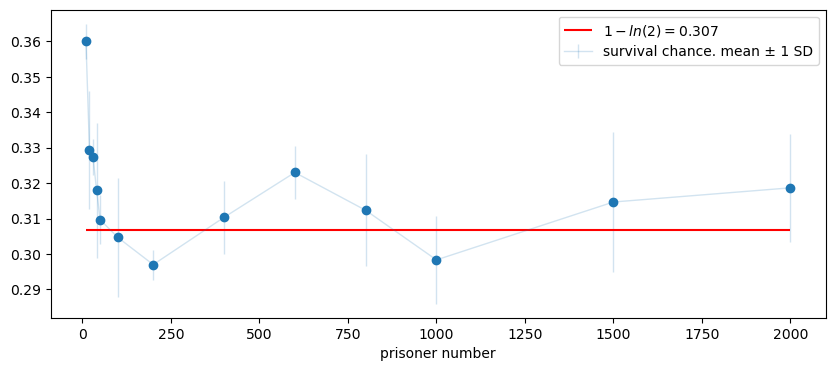
\includegraphics[width=0.6\textwidth]{fig1-locker2.png}
    \caption{Survival chance against prisoner number (n). When n is large enough, this chance will approach 1-ln2.}
    \label{fig:locker2}
\end{figure}

\subsection{Galton Board}
The binomial distribution originates from the repeated independent Bernoulli trials.
Its PMF (probability mass function) is defined as $P(x=k)=C_{n}^{k}p^{k}(1-p)^{n-k},k=0,1,...,n$,
n is the trial number. p is the probability of interest event in each Bernoulli trial.
The Galton board, a.k.a. quincunx or bean machine, is a historical device to demonstrate
the binomial distribution. mc-tk provides a Binom class to simulate this experiment (Figure \ref{fig:galton board mc}).

\lstset{
    basicstyle=\footnotesize,
    xleftmargin=-3em,aboveskip=0.5em,aboveskip=0.5em
}
\begin{lstlisting}[language=python]
      Galton_Board(n=20, N=5000, flavor=1).run()
      # n : the number of nail plate layers.
      # N : how many MC experiments to run.
      # flavor : 1 or 2. Which implementation to use.
      \end{lstlisting}

\begin{figure}[htbp]
    \centering
    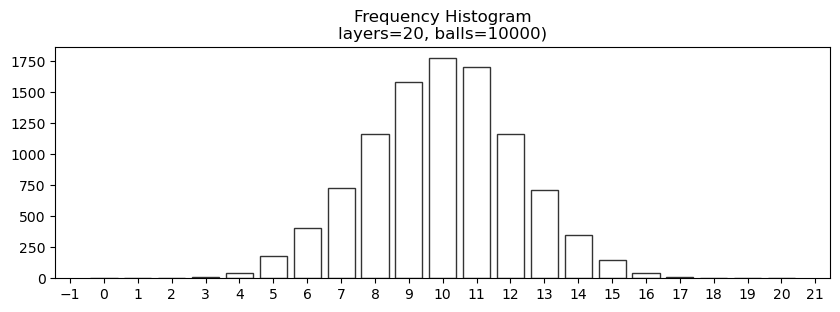
\includegraphics[width=0.49\textwidth]{fig2-galton board mc1.png}
    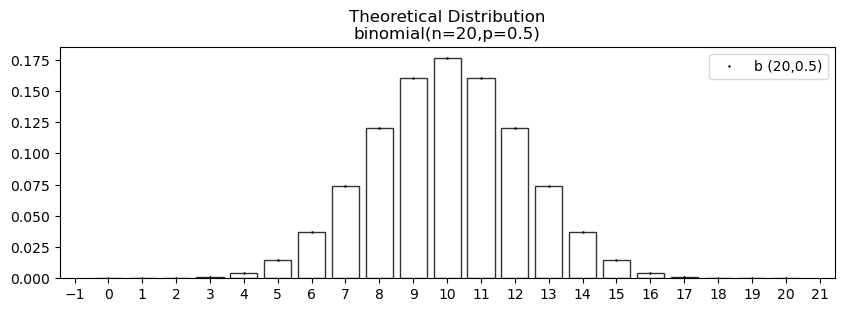
\includegraphics[width=0.49\textwidth]{fig2-galton board mc2.png}
    \caption{Use the Galton board MC experiment (10000 balls, 20 layers) to reproduce the binomial distribution.}
    \label{fig:galton board mc}
\end{figure}

\subsection{Survival Game}
The exponential distribution describes a continuous random variable with the following PDF
(probability density function):

\begin{equation}
    \label{deqn_ex1}
    p(x)= \left\{\begin{array}{rcl}
        \theta e^{-\theta x}, & x > 0    \\
        0,                    & x \leq 0 \\
    \end{array}\right.
    (\theta > 0)
\end{equation}

In mc-tk, we define a survival game to illustrate the underlying mechanism of the exponential
distribution. Because the sudden death game can approximate many real-life accidents or
electronic component failures (e.g., capacity breakdown or LCD pixel defect), the resulting
exponential distribution can be used in survival analysis and lifespan estimation.

In each round of this survival game, the test subject (player) is faced with a very
low sudden death probability (p). In Figure \ref{fig:exponential mc}, we choose p = 0.001 and
simulate 10,000 MC rounds. The generated histogram is very close to the exponential distribution.
This class can be used to illustrate the generation mechanism of the exponential distribution.

\lstset{
    basicstyle=\footnotesize,
    xleftmargin=-3em,aboveskip=0.5em,belowskip=0.5em
}
\begin{lstlisting}[language=python]
      Sudden_Death(n=1000,p=0.01,N=10000).run()
      # n : the rounds of survival games.
      # p : the probability of sudden death/failure/accident in each round.
      # N : how many MC experiments to run.
      \end{lstlisting}

\begin{figure}[htbp]
    \centering
    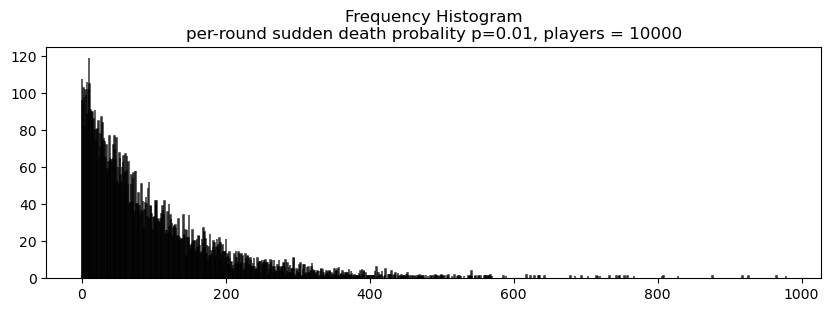
\includegraphics[width=0.49\textwidth]{fig3-exponential mc1.png}
    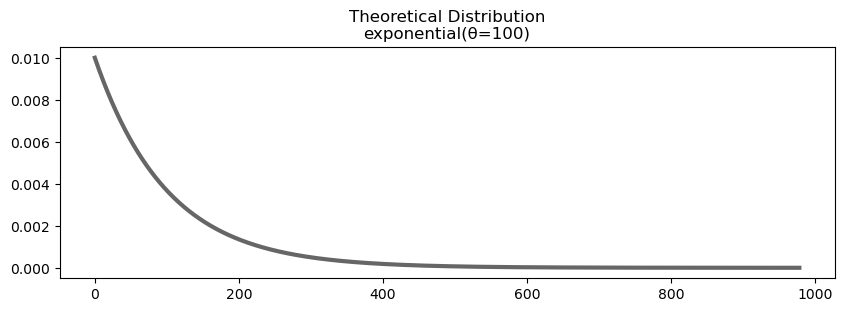
\includegraphics[width=0.49\textwidth]{fig3-exponential mc2.png}
    \caption{The observed frequency histogram of the survival game and the corresponding theoretical exponential distribution.}
    \label{fig:exponential mc}
\end{figure}

\subsection{Paper Clip Experiment}
The Zipf law was proposed by George Kingsley Zipf in 1949 from his linguistic research \cite{bib14}.
The Zipf law says that a word's frequency in natural language is inversely proportional
to its rank. This means only a few words are frequently used, and most are seldom used.
This phenomenon is known as the 80/20 law, the long tail distribution, or the Pareto principle.
The PDF of the Zipf distribution is as follows.

\begin{equation}
    \label{deqn_ex2}
    p(k;a)=\frac{1}{\zeta(a)k^{a}}
\end{equation}

$k \geq 1$,$a > 1$. a is the shape parameter. $\zeta$ is the Riemann zeta function,
which is defined as:
\begin{equation}
    \label{deqn_ex3}
    \zeta(x)=\sum_{n=1}^{\infty}(\frac{1}{n^x})=\sum_{n=1}^{\infty}n^{-x}=\frac{1}{1^x}+\frac{1}{2^x}+\frac{1}{3^x}+\frac{1}{4^x}+...
\end{equation}

It has many interesting properties, e.g.,
\begin{equation}
    \label{deqn_ex4}
    \zeta(1)=\frac{1}{1}+\frac{1}{2}+\frac{1}{3}+\frac{1}{4}+...=+\infty
\end{equation}
\begin{equation}
    \label{deqn_ex5}
    \zeta(2)=\frac{1}{1^2}+\frac{1}{2^2}+\frac{1}{3^2}+\frac{1}{4^2}+...=\frac{\pi^2}{6}
\end{equation}
\begin{equation}
    \label{deqn_ex6}
    \zeta(-1)=1+2+3+4+...=-\frac{1}{12}
\end{equation}
\begin{equation}
    \label{deqn_ex7}
    \zeta(-2)=1^2+2^2+3^2+4^2+...=0
\end{equation}

The MC experiment related to the Zipf distribution is the paper clip experiment.
Each time, we drew two clips from a pipe of paper clips. The picked clips are
connected and then put back. After enough rounds, the clip chains of different
lengths will obey the Zipf distribution. Users may call the Paper\_Clips class
to simulate this experiment (Figure \ref{fig:zipf mc}).

\lstset{
    basicstyle=\footnotesize,
    xleftmargin=-3em,aboveskip=0.5em,belowskip=0.5em
}
\begin{lstlisting}[language=python]
      Zipf(N=10000,n=16000).run()
      # N : the number of rounds in the paper clip experiment.
      # n : the total number of paper clips. It should always be greater than [num_rounds].
      \end{lstlisting}

\begin{figure}[htbp]
    \centering
    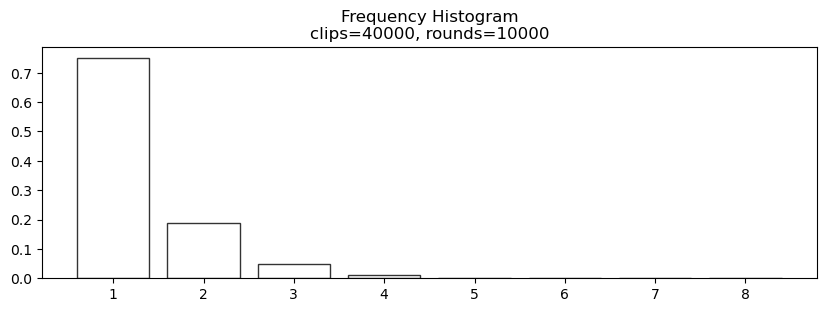
\includegraphics[width=0.49\textwidth]{fig4-zipf mc1.png}
    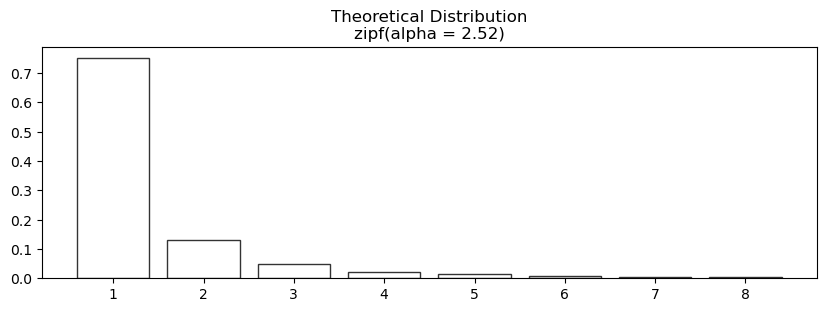
\includegraphics[width=0.49\textwidth]{fig4-zipf mc2.png}
    \caption{Use the paper clip MC experiment to generate the Zipf distribution.}
    \label{fig:zipf mc}
\end{figure}

\section{Classes for common distributions}
The "distributions" module provides MC experiment to generate specific distributions.
The observed MC result and theoretical distribution PDF/PMF are provided side by side.

\subsection{Poisson Distribution}
The Poisson distribution has the following PMF:$P(X=k)=\frac{\lambda^k}{k!}e^{-\lambda},k=0,1,...,\lambda>0$.
Many daily-life events follow the Poisson distribution, e.g., the car accidents that happen every day,
the patient visits in the emergency department, etc. The Poisson distribution can be seen as a particular
case of the binomial distribution when p is very low and n is very large. Figure \ref{fig:possion mc} demonstrates the
Poisson class in mc-tk. In each MC round, a large sample size (n = 10000) is used, and each individual
is faced with an extremely low accident probability (p = 0.0001). By simulating 100000 MC rounds, we can see
that the total number of accidents follows a perfect Poisson distribution.

\lstset{
    basicstyle=\footnotesize,
    xleftmargin=-1em,aboveskip=0.5em,belowskip=0.5em
}
\begin{lstlisting}[language=python]
    Poisson(n=10000,p=0.0001,N=100000).run()
    # n,p : the params of binom, i.e., b(n,p)
    # N : how many MC experiments to run.
    \end{lstlisting}

\begin{figure}[htbp]
    \centering
    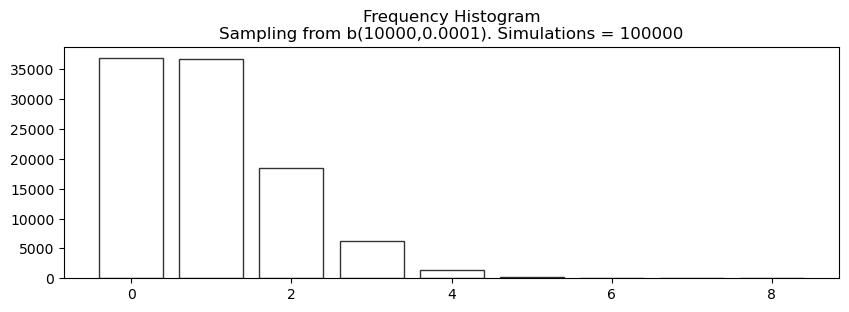
\includegraphics[width=0.46\textwidth]{fig5-poisson mc1.png}
    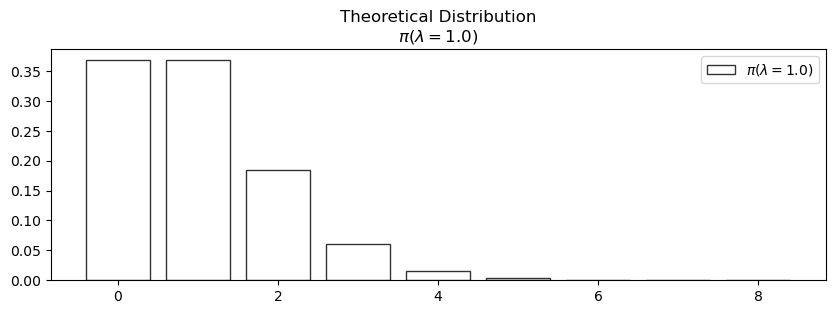
\includegraphics[width=0.46\textwidth]{fig5-poisson mc2.png}
    \caption{The observed frequency histogram of 100,000 random samples drawn from b(10000, 0.0001) and the corresponding theoretical Poisson distribution.}
    \label{fig:possion mc}
\end{figure}

\subsection{Benford Distribution}
The Benford law, a.k.a. the Newcomb-Benford law or the first-digit law, describes the PMF of
leading digits in many real-life financial and social data \cite{bib15}. In essence, the natural or social
processes that follow the power laws (very common) often demonstrate this distribution.
Financial audits often use it to check faked or manipulated data. The Benford PMF is as follows (Table \ref{tab:benford p}).

\begin{table}[htbp] \footnotesize
    \centering
    \caption{Leading digit PMF}\label{tab:benford p}
    \begin{tabular}{cccccccccc}
        \hline
        leading digit & 1      & 2      & 3      & 4     & 5     & 6     & 7     & 8     & 9     \\
        p             & 30.1\% & 17.6\% & 12.5\% & 9.7\% & 7.9\% & 6.7\% & 5.8\% & 5.1\% & 4.6\% \\
        \hline
    \end{tabular}
\end{table}

The Benford class provides three examples to verify the Benford law (Figure \ref{fig:benford mc}).
The first example uses the 20-year trading volume data of AAPL (Apple Inc.). The second example
uses the United Nations' international trading data. The last example uses the Fibonacci series.

\lstset{
    basicstyle=\footnotesize,
    xleftmargin=-1em,aboveskip=0.5em,belowskip=0.5em
}
\begin{lstlisting}[language=python]
    Benford(data="stock",N=1000).run()
    # data : data set to be used.
    #  'stock' - use 20-year stock trading volume data of Apple Inc. (AAPL)
    #  'trade' - use annual trade data from various countries. https://comtrade.un.org/data/mbs
    #  'fibonacci' - use the top-N fibonacci series.    
    # N : how many MC experiments to run.
    \end{lstlisting}

According to Figure \ref{fig:benford mc}, all the examples fit well against the theoretical Benford distribution.
We can use the Fibonacci series to explain the Benford law intuitively. The Fibonacci sequence
represents how a population (e.g., rabbits) grows in a resource-unlimited environment.
At a steady breeding speed, it takes much longer time to increase the population from 100 to 200
(need to increase by 100) than from 90 to 100 (only need to increase by 10). It also takes longer
time than 200 to 300 because the population has grown bigger in the latter case. Therefore, it stays longer
at smaller leading digits than the bigger ones.

\begin{figure}[htbp]
    \centering
    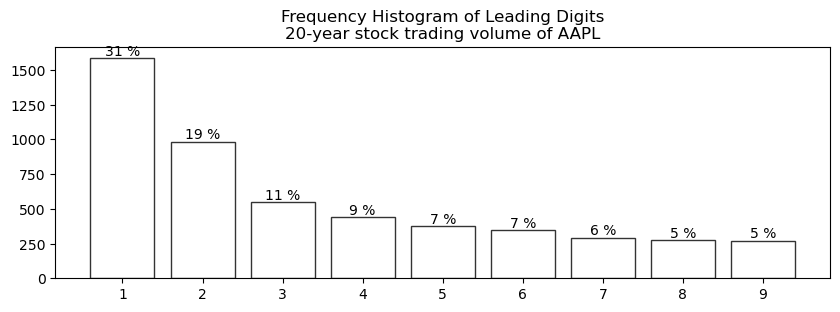
\includegraphics[width=0.47\textwidth]{fig6-benford mc1.png}
    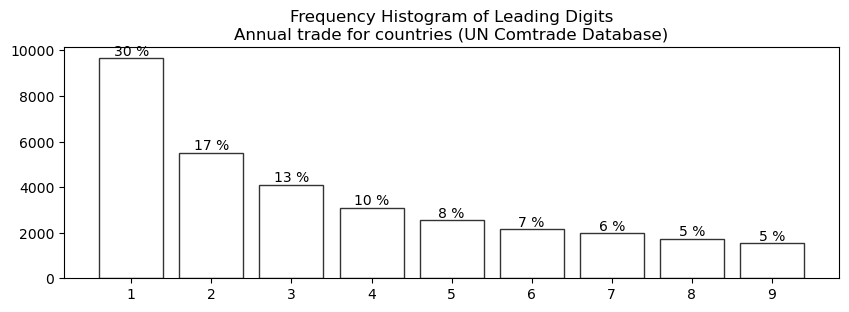
\includegraphics[width=0.47\textwidth]{fig6-benford mc2.png}
    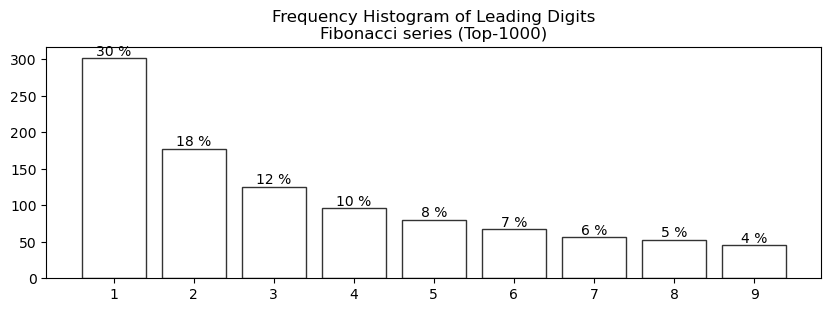
\includegraphics[width=0.47\textwidth]{fig6-benford mc3.png}
    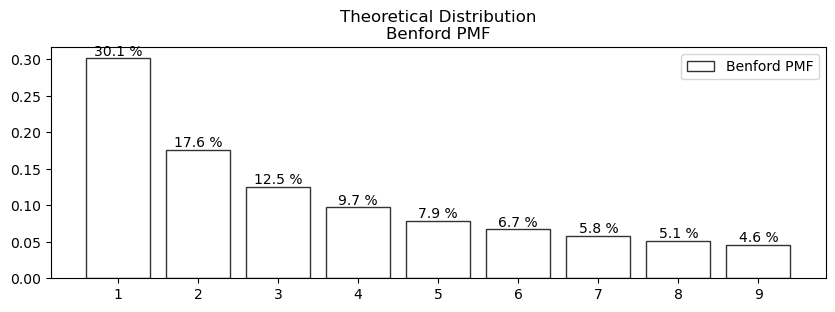
\includegraphics[width=0.47\textwidth]{fig6-benford mc4.png}
    \caption{Verify the Benford law using two real-life datasets and the Fibonacci series.}
    \label{fig:benford mc}
\end{figure}

\vspace{-1em}
\section{Classes for sampling distributions}
The "samplings" module provides classes to verify the sampling of common hypothesis testing statistics(Table \ref{tab:sampling}).
Each class constructs the test statistic's random variable and compares it with the theoretical sampling distribution.


\begin{sidewaystable}[htbp] \small
    \centering
    \caption{Sampling distributions for commonly used hypothesis tests} \label{tab:sampling}
    \begin{tabular}{c|c|c|c|c}
        \hline
        mc-tk class                                                                              & \begin{tabular}[c]{@{}c@{}}Statistical Testing \\Task\end{tabular}       & \begin{tabular}[c]{@{}c@{}}$H_0$ and population \\distribution\end{tabular}                         & Test Statistic                                                                                                             & Sampling distribution           \\
        \hline
        \begin{tabular}[c]{@{}c@{}}samplings.\\T\_Test\end{tabular}                              & Student's t test                                                         & $H_0:\mu = \mu_0$                                                                                   & $t=\frac{\overline{x}-\mu}{\frac{S}{\sqrt{n}}}$                                                                            & $t(n-1)$                        \\
        \hline
        \begin{tabular}[c]{@{}c@{}}samplings.\\Chisq\_Gof\_Test\end{tabular}                     & \begin{tabular}[c]{@{}c@{}}Pearson's Chi\\-squared GOF Test\end{tabular} & $H_0:PMF_1 = PMF_2$                                                                                 & $\chi^2=\sum_{j=1}^k\frac{(f_j-np_j)^2}{np_j}$                                                                             & $\chi^2(k-1)$                   \\
        \hline
        \begin{tabular}[c]{@{}c@{}}samplings.\\Anova\end{tabular}                                & ANOVA                                                                    & $H_0:\mu_1=\mu_2=...=\mu_k$                                                                         & $F=\frac{MSTR}{MSE}$                                                                                                       & $F(k-1,n-1)$                    \\
        \hline
        \begin{tabular}[c]{@{}c@{}}samplings.\\Kw\_Test\end{tabular}                             & Kruskal-Wallis                                                           & \begin{tabular}[c]{@{}c@{}}$H_0$:All k populations \\have the same median\end{tabular}              & $H=[\frac{12}{n_T(n_T+1)}\sum_{i=1}^{k}\frac{R_{i}^2}{n_i}]-3(n_T+1)$                                                      & $\chi^2(k-1)$                   \\
        \hline
        \begin{tabular}[c]{@{}c@{}}samplings.\\Fk\_Test\end{tabular}                             & Fligner-Killeen Test                                                     & \begin{tabular}[c]{@{}c@{}}$H_0$:All k population \\variances are equal\end{tabular}                & $FK=\frac{\sum_{j=1}^{k}n_j(\overline{a_j}-\overline{a})^2}{s^2}$                                                          & $\chi^2(k-1)$                   \\
        \hline
        \begin{tabular}[c]{@{}c@{}}samplings.\\Bartlett\_Test\end{tabular}                       & Bartlett's Test                                                          & \begin{tabular}[c]{@{}c@{}}$H_0$:All k population \\variances are equal\end{tabular}                & $\chi^2=\frac{(N-k)ln(S_p^2)-\sum_{i=1}^k(n_i-1)ln(S_i^2)}{1+\frac{1}{3(k-1)}(\sum_{i=1}^k(\frac{1}{n_i})-\frac{1}{N-k})}$ & $\chi^2(k-1)$                   \\
        \hline
        \begin{tabular}[c]{@{}c@{}}samplings.\\Sign\_Test\end{tabular}                           & sign test                                                                & $H_0:m = m_0$                                                                                       & N- \qquad N+                                                                                                               & $b(n,p)$                        \\
        \hline
        \begin{tabular}[c]{@{}c@{}}samplings.\\Cochrange\_Q\_Test\end{tabular}                   & Cochran Q Test                                                           & \begin{tabular}[c]{@{}c@{}}$H_0$:No difference between the \\k~dichotomous populations\end{tabular} & $T=\frac{(k-1)[k\sum_{j=1}^kX_{.j}^2-(\sum_{j=1}^kX_{.j})^2]}{k\sum_{i=1}^bX_{i.}-\sum_{i=1}^bX_{i.}^2}$                   & $\chi^2(k-1)$                   \\
        \hline
        \begin{tabular}[c]{@{}c@{}}samplings.\\Median\_Test\end{tabular}                         & Median Test                                                              & \begin{tabular}[c]{@{}c@{}}$H_0$:All k populations \\have the same median\end{tabular}              & $MT=\frac{N^2}{ab}\sum_{i=1}^{k}\frac{(O_{1i}-n_{i}a/N)^2}{n_{i}}$                                                         & $\chi^2(k-1)$                   \\
        \hline
        \multirow{2}{*}{\begin{tabular}[c]{@{}c@{}}samplings.\\Hotelling\_T2\_Test\end{tabular}} & \multirow{2}{*}{Hotelling T\textsuperscript{2 }Test}                     & $H_0:\mu_1=\mu2$                                                                                    & \multirow{2}{*}{$T^2=n(\overline{x}-\mu)^TS^{-1}(\overline{x}-\mu)$}                                                       & \multirow{2}{*}{$T^2(k,n_k-1)$} \\
                                                                                                 &                                                                          & $\mu_1$ and $\mu_2$ are vectors                                                                     &                                                                                                                            &                                 \\
        \hline
        \begin{tabular}[c]{@{}c@{}}samplings.\\Clt\end{tabular}                                  & Central Limit Theorem                                                    & $x_1,x_2,...,x_n$ are n i.i.d. r.v.s.                                                               & $\overline{x}=\frac{x_1+x_2+...+x_n}{n}$                                                                                   & $N(\mu,\sigma^2)$               \\
        \hline
    \end{tabular}
\end{sidewaystable}

\subsection{Student's t test}
In T\_Test class, we sample n samples from a normal distribution, the
statistic will follow the student's distribution(Figure \ref{fig:t mc}).

\begin{equation}
    \label{deqn_ex8}
    \frac{\overline{x}-\mu}{\frac{S}{\sqrt{n}}} \sim t(n-1)
\end{equation}


\lstset{
    basicstyle=\footnotesize,
    xleftmargin=-1em,aboveskip=0.5em,belowskip=0.5em
}
\begin{lstlisting}[language=python]
    T_Test(n=10,N=10000).run()    
    # n : sample size.
    # N : how many MC experiments to run.
    \end{lstlisting}

\begin{figure}[htbp]
    \centering
    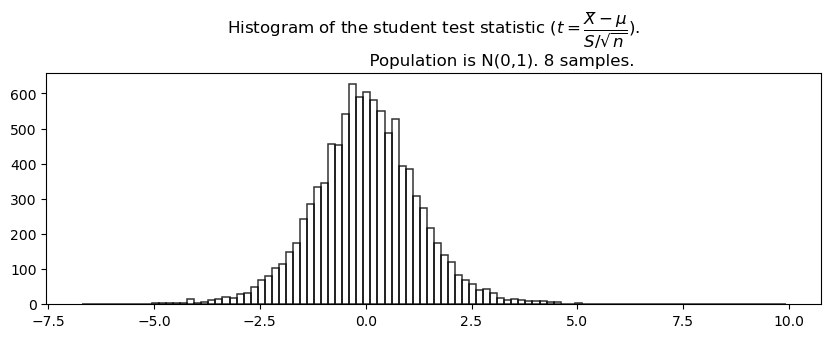
\includegraphics[width=0.45\textwidth]{fig7-t mc1.png}
    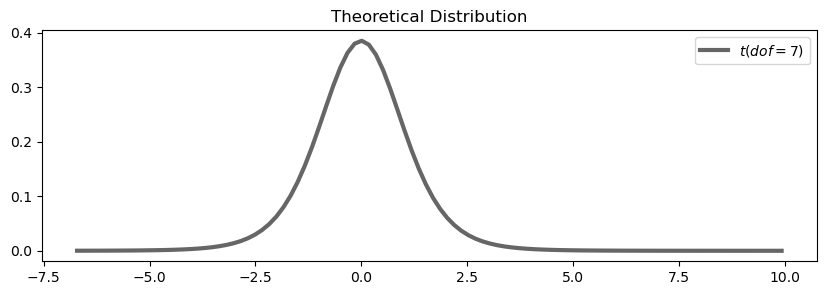
\includegraphics[width=0.45\textwidth]{fig7-t mc2.png}
    \caption{The observed frequency histogram and the corresponding theoretical t distribution.}
    \label{fig:t mc}
\end{figure}

\subsection{Pearson's Chi-Square Goodness-of-Fit Test}
Pearson's Chi-Square Goodness-of-Fit (GOF) test uses the following statistic.
\begin{equation}
    \label{deqn_ex9}
    \chi^2=\sum_{j=1}^{k}\frac{(f_{j}-np_{j})^2}{np_{j}} \sim \chi^2(k-1)
\end{equation}

When n is large enough ($n \geq 50$), $\chi^2$ will follow the $\chi^2(k-1)$ distribution.
As Pearson's chi-square GOF test is non-parametric, there is no restriction on the population distribution.
The Chisq\_Gof\_Test class provides two population distributions. (1) The first is the Galton board (use the binominal
population, Figure \ref{fig:galton gof}). (2) The second is the dice game (use the uniform PMF, Figure \ref{fig:dice gof}). In both cases,
the statistic histogram from the MC experiment is very close to the theoretical $\chi^2(k-1)$ distribution.

\lstset{
    basicstyle=\footnotesize,
    xleftmargin=-1em,aboveskip=0.5em,belowskip=0.5em
}
\begin{lstlisting}[language=python]
    Chisq_Gof_Stat(underlying_dist='binom',k=8,sample_size=100,N=10000).run()
    # underlying_dist : what kind of population dist to use. By default, 
    #                   we use binom, i.e., the Galton board.
    #   'binom'/'galton' - the population is binom.
    #   'dice' - 6 * 1/6.
    # k : classes in the PMF.
    # N : how many MC experiments to run.
    \end{lstlisting}

\begin{figure}[htbp]
    \centering
    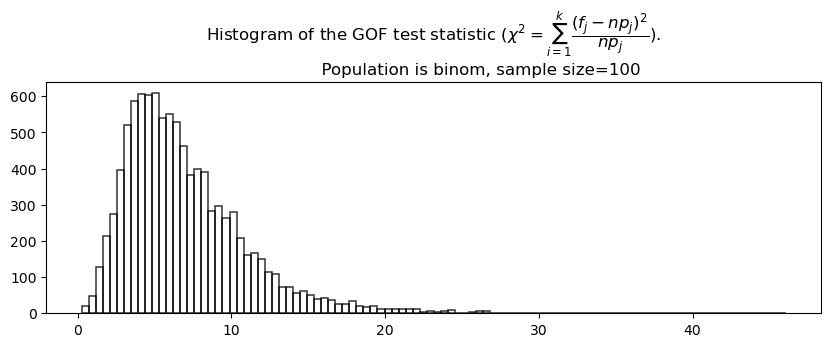
\includegraphics[width=0.45\textwidth]{fig8-galton gof1.png}
    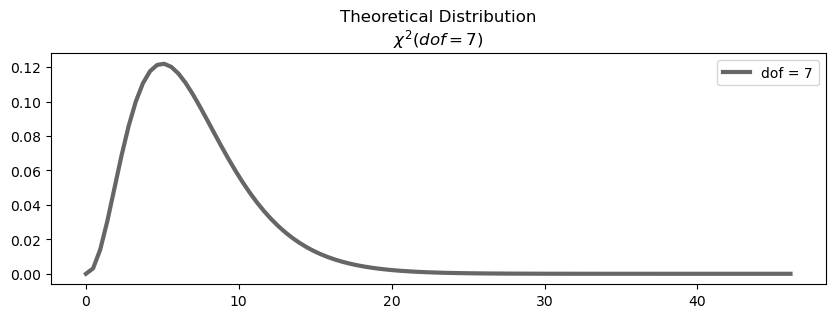
\includegraphics[width=0.45\textwidth]{fig8-galton gof2.png}
    \caption{Use the Galton Board game to verify the statistic in Pearson's chi-square GOF test.}
    \label{fig:galton gof}
\end{figure}

\begin{figure}[htbp]
    \centering
    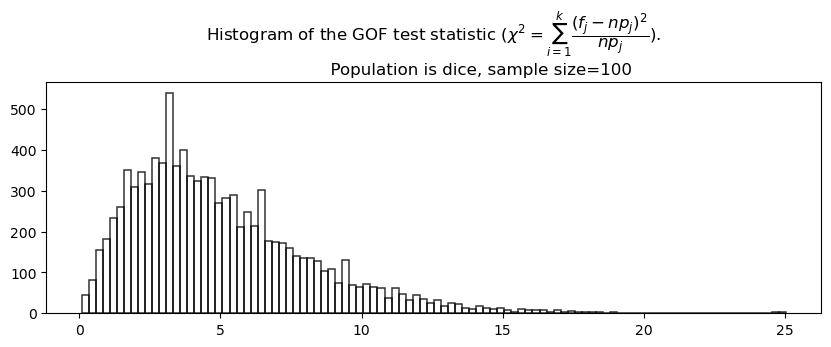
\includegraphics[width=0.45\textwidth]{fig9-dice gof1.png}
    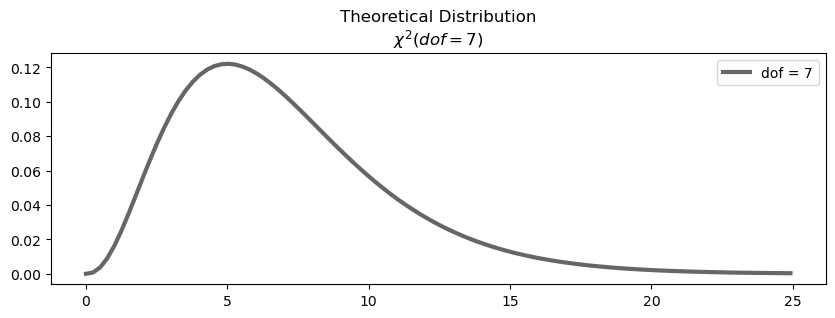
\includegraphics[width=0.45\textwidth]{fig9-dice gof2.png}
    \caption{Use the dice game to verify the statistic in Pearson's chi-square GOF test.}
    \label{fig:dice gof}
\end{figure}

\subsection{ANOVA}
ANOVA (analysis of variance) is a parametric mean test for multiple groups. Its null hypothesis $H_{0}$ is: $\mu_{1}=\mu_{2}=...=\mu_{k}$.
ANOVA constructs the test statistic by splitting the total variance into treatment (between-class difference, MSTR) and noise (within-class variance, MSE).
When $H_{0}$ is true, the ratio of MSTR and MSE will follow the F distribution, i.e., $F=\frac{MSTR}{MSE} \sim F(k-1,n-1)$.

The Anova class will calculate the histogram of the F statistic observed from a multi-group normal sample (Figure \ref{fig:anova mc}).

\lstset{
    basicstyle=\footnotesize,
    xleftmargin=-1em,aboveskip=0.5em,belowskip=0.5em
}
\begin{lstlisting}[language=python]
    Anova(k=10,n=10,N=10000).run()
    # k : the number of classes/groups.
    # n : the sample size in each class/group. The total sample size is [k]*[n].
    # N : how many MC experiments to run.
    \end{lstlisting}

\begin{figure}[htbp]
    \centering
    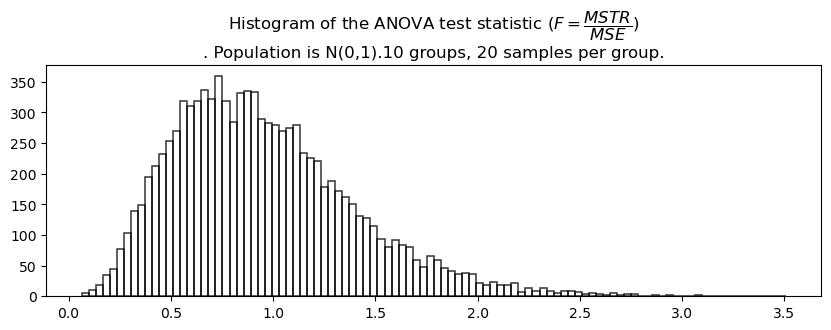
\includegraphics[width=0.46\textwidth]{fig10-anova mc1.png}
    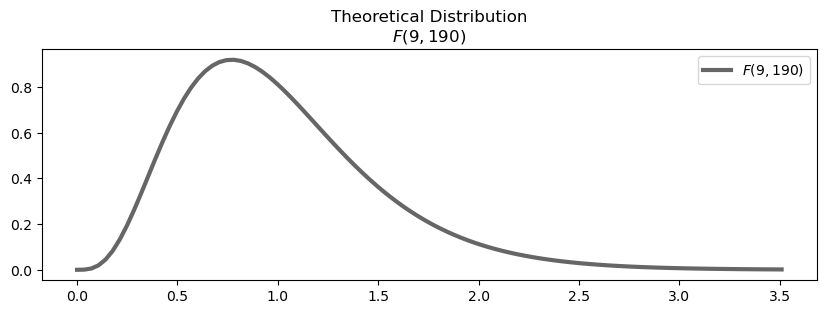
\includegraphics[width=0.48\textwidth]{fig10-anova mc2.png}
    \caption{Use MC to verify the ANOVA test statistic follows the F distribution.}
    \label{fig:anova mc}
\end{figure}

\subsection{Kruskal-Wallis test}
Kruskal-Wallis (K-W test) is the non-parametric counterpart for ANOVA. It can be applied to non-normal
populations. Kruskal-Wallis is also an extension to the non-parametric Mann-Whitney or Wilcoxon rank sum test.
The latter compares two groups, while Kruskal-Wallis can compare three or more.

The null hypothesis of the K-W test assumes that all populations have the same median.
K-W is a rank-based test. Its H statistic is defined as:

\begin{equation}
    \label{deqn_ex10}
    H=[\frac{12}{n_{T}(n_{T}+1)}\sum_{i=1}^{k}\frac{R_{i}^{2}}{n_{i}}]-3(n_{T}+1)
\end{equation}

\noindent k is number of populations. $n_{i}$ is the number of observations in group/sample I,
$n_{T}=\sum_{i=1}^{k}n_{i}$ is the total number of observations in all samples.
$R_{i}$ is the sum of the ranks for sample i.

The Kw\_Test class verifies that H follows the chi-square distribution (Figure \ref{fig:kw mc}).

\lstset{
    basicstyle=\footnotesize,
    xleftmargin=-1em,aboveskip=0.5em,belowskip=0.5em
}
\begin{lstlisting}[language=python]
    Kw_Test(underlying_dist='uniform',k=3,n=100,N=10000).run()
    # underlying_dist : population assumption. As the KW test is non-parametric, 
    #     the choice of dist doesn't matter. By default, we use uniform.
    # k : the number of groups/classes.
    # n : samples per class. In this experiment, we use equal group size, i.e., n1=n2=n3=...
    # N : how many MC experiments to run.
    \end{lstlisting}

\begin{figure}[htbp]
    \centering
    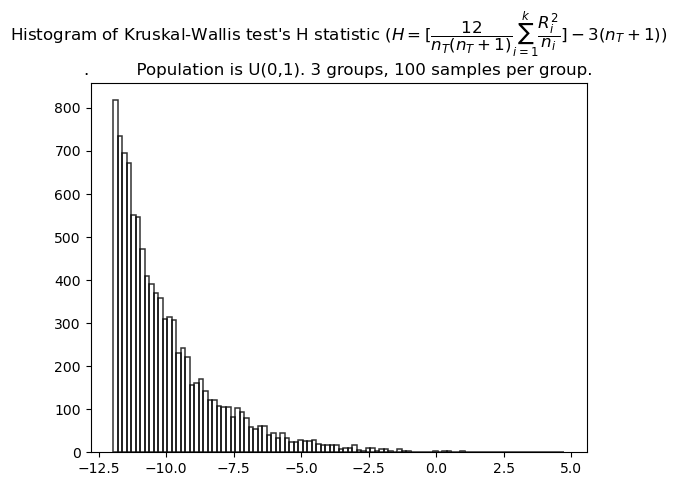
\includegraphics[width=0.54\textwidth]{fig11-kw mc1.png}
    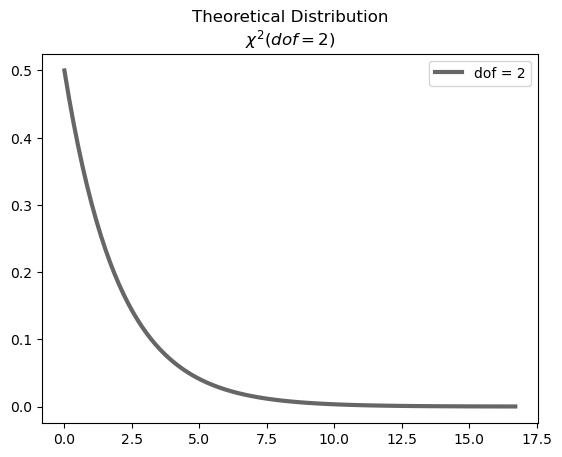
\includegraphics[width=0.45\textwidth]{fig11-kw mc2.png}
    \caption{The Kruskal Wallis H statistic follows the chi-square distribution.}
    \label{fig:kw mc}
\end{figure}

\subsection{Fligner-Killeen Test}
The Fligner-Killeen test is a non-parametric test for homogeneity of group variances
based on ranks. It is a robust HOV (homogeneity of variances) test against departures from normality.
It is more robust than the Levene test. The Fligner Killeen statistic is $FK=\frac{\sum_{j=1}^{k}n_{j}(\overline{a_{j}}-\overline{a})^2}{s^2}$,
k is the number of groups, $n_{j}$ is the size of the $j^{th}$ group, $\overline{a_{j}}$ is the group mean, $\overline{a}$ is the grand mean and
$s^2$ is the grand variance. The Fk\_Test class verifies the FK statistic follows the chi-square sampling distribution (Figure \ref{fig:fk mc}).

\lstset{
    basicstyle=\footnotesize,
    xleftmargin=-1em,aboveskip=0.5em,belowskip=0.5em
}
\begin{lstlisting}[language=python]
    Fk_Test(n=10,k=5,N=1000).run()
    # n : the sample size in each group/class. In this experiment, all group sizes are equal.    
    # k : the number of groups/classes.
    # N : how many MC experiments to run.
    \end{lstlisting}

\begin{figure}[htbp]
    \centering
    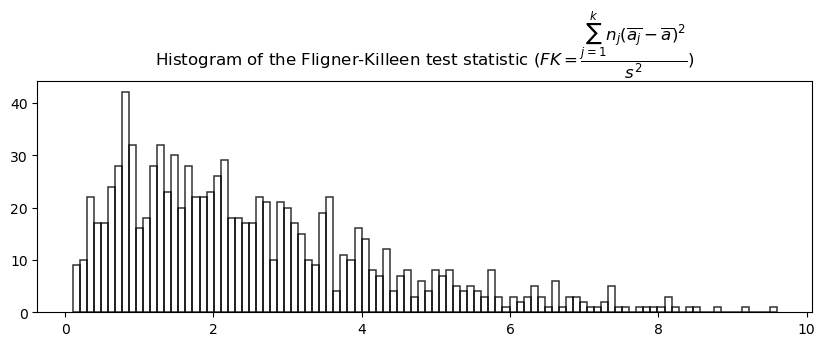
\includegraphics[width=0.45\textwidth]{fig12-fk mc1.png}
    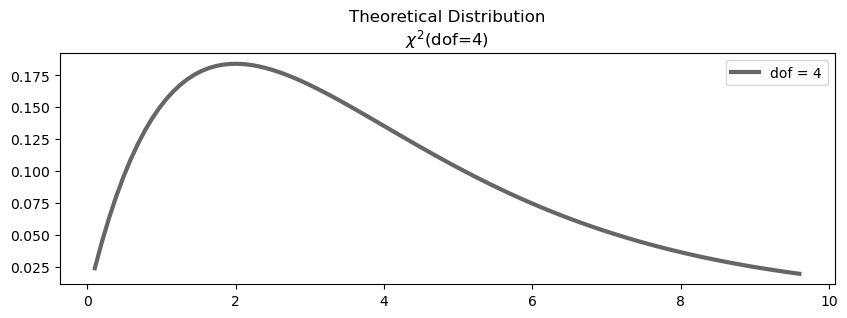
\includegraphics[width=0.45\textwidth]{fig12-fk mc2.png}
    \caption{The observed histogram and theoretical distribution of the Fligner-Killeen statistic.}
    \label{fig:fk mc}
\end{figure}

\subsection{Bartlett's Test}
Bartlett's test is another HOV test. Bartlett's test is sensitive to departures from normality.
Its test statistic is as follows.
\begin{equation}
    \label{deqn_ex11}
    \chi^2=\frac{(N-k)ln(S_p^2)-\sum_{i=1}^k(n_i-1)ln(S_i^2)}{1+\frac{1}{3(k-1)}(\sum_{i=1}^k(\frac{1}{n_i})-\frac{1}{N-k})}
\end{equation}


Where k is the group number. $n_{i}$ and $S_{i}^2$ are the $i{th}$ group size and variance.
$N=\sum_{i=1}^{k}n_{i}$ is the grand total. $S_{P}^{2}=\frac{1}{N-k}\sum_{i}(n_{i}-1)$. $S_{i}^2$ is the pooled variance.

mc-tk provides the Bartlett\_Test class to verify the test statistic follows a distribution (Figure \ref{fig: bartlett mc}).

\lstset{
    basicstyle=\footnotesize,
    xleftmargin=-1em,aboveskip=0.5em,belowskip=0.5em
}
\begin{lstlisting}[language=python]
    Bartlett_Test(k=5,n=10,N=1000).run()
    # k : the number of groups/classes.
    # n : the sample size in each group/class. In this experiment, all group sizes are equal.     
    # N : how many MC experiments to run.
    \end{lstlisting}

\begin{figure}[htbp]
    \centering
    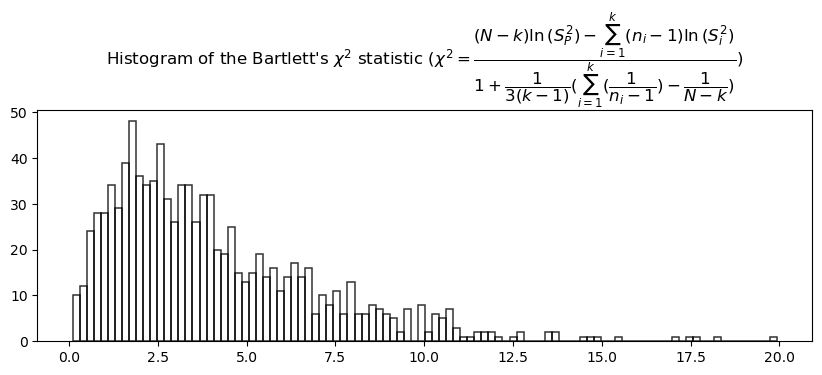
\includegraphics[width=0.48\textwidth]{fig13-bartlett mc1.png}
    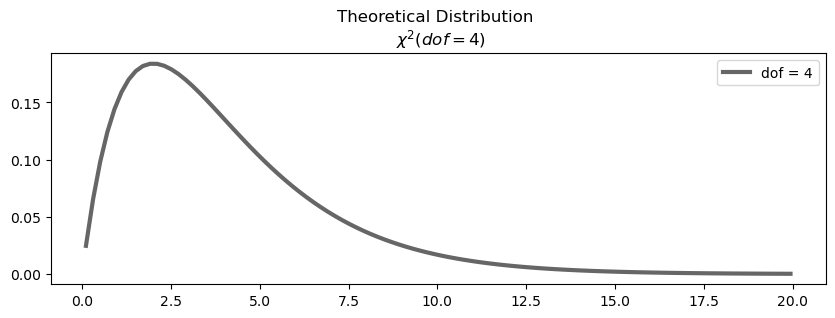
\includegraphics[width=0.43\textwidth]{fig13-bartlett mc2.png}
    \caption{The observed histogram and theoretical distribution of Bartlett's test statistic.}
    \label{fig: bartlett mc}
\end{figure}

\subsection{Sign Test}
The sign test is a widely used non-parametric median test. The sign test first subtracts each sample
by the grand median, i.e., $X_{i}-m_{0}$,$i=1,2,...,n$. Then, it counts positive and negative numbers
denoted as N+ and N-. If the null hypothesis ($H_{0}:m=m_{0}$) is true, N+ and N- will both follow
binomial distributions:
\begin{equation}
    \label{deqn_ex12}
    N- \sim b(n,\frac{1}{2}) \qquad  N+ \sim b(n,\frac{1}{2})
\end{equation}

To verify this sampling distribution, we can use the Sign\_Test class. This class uses
the exponential distribution for demonstration. By solving $\int_{m}^{\infty}\theta e^{-\theta x}dx = 1/2$,
we can get the theoretical median is $m=\theta ln^{(2)}$. The Sign\_Test class draws samples
from the exponential population and compares each sample with the theoretical median to get the N+ and N-
statistic values. The result is shown in Figure \ref{fig:sign mc}.

\lstset{
    basicstyle=\footnotesize,
    xleftmargin=-1em,aboveskip=0.5em,belowskip=0.5em
}
\begin{lstlisting}[language=python]
    Sign_Test(underlying_dist='expon',n=100,N=10000).run()
    # underlying_dist : population assumption. As the sign test is non-parametric, 
    #        the choice of dist doesn't matter. By default, we use exponential. 
    # n : sample size.
    # N : how many MC experiments to run.
    \end{lstlisting}

\begin{figure}[htbp]
    \centering

    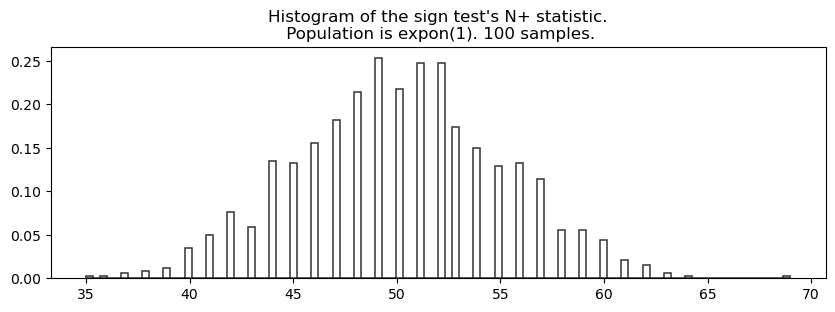
\includegraphics[width=0.32\textwidth]{fig14-sign mc1.png}
    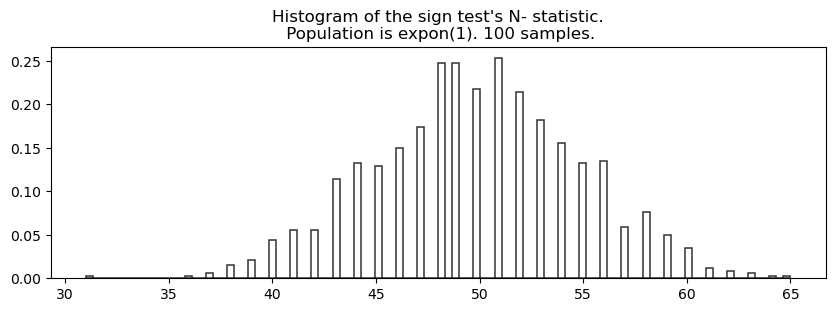
\includegraphics[width=0.32\textwidth]{fig14-sign mc2.png}
    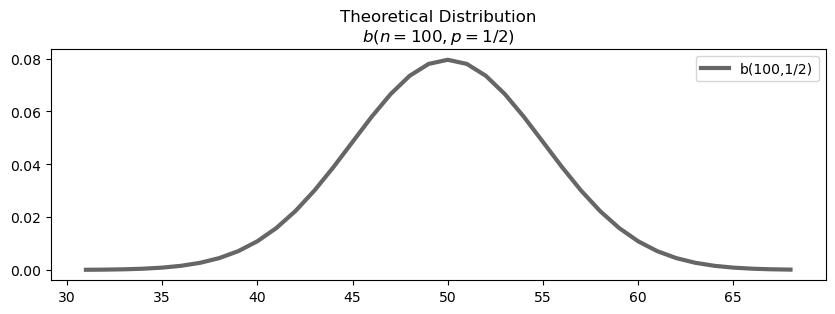
\includegraphics[width=0.32\textwidth]{fig14-sign mc3.png}
    \caption{Use the exponential distribution to verify the N+ and N- follow the binomial distributions.}
    \label{fig:sign mc}
\end{figure}

\subsection{Cochrane-Q Tes}
The Cochran's Q test is a non-parametric test to check whether three or more dichotomous / Boolean groups have the same True or False proportions.
This test uses the T statistic.
\begin{equation}
    \label{deqn_ex13}
    T = \frac{(k-1)[k\sum_{j=1}^{k}X_{.j}^{2}-(\sum_{j=1}^{k}X_{.j})^2]}{k\sum_{i=1}^{b}X_{i.}-\sum_{i=1}^{b}X_{i.}^2}
\end{equation}

\noindent k: The number of treatments / groups \\
$X_{.j}$: The column total for the  treatment \\
b: The number of rows (i.e., samples per class) \\
$X_{i.}$: The total for the $i^{th}$ row \\
N: The grand total

The Cochrane\_Q\_Test class verifies T follows the $\chi^2(k-1)$ distribution.
Because Cochrane's Q requires Boolean data, the Cochrane\_Q\_Test class uses the Bernoulli distribution
to generate samples (Figure \ref{fig:Cochran Q mc}).

\lstset{
    basicstyle=\footnotesize,
    xleftmargin=-1em,aboveskip=0.5em,belowskip=0.5em
}
\begin{lstlisting}[language=python]
    Cochrane_Q_Test(p=0.5,k=3,n=100,N=10000).run()
    # p : we draw from a Bernoulli population with p. p is the "success/pass" probability.
    # k : the number of groups/classes.
    # n : the sample size in each group/class. In this experiment, all group sizes are equal,
    #     as Cochrane-Q is paired / dependent.
    # N : how many MC experiments to run.
    \end{lstlisting}

\begin{figure}[htbp]
    \centering
    \vspace{-0.5em}

    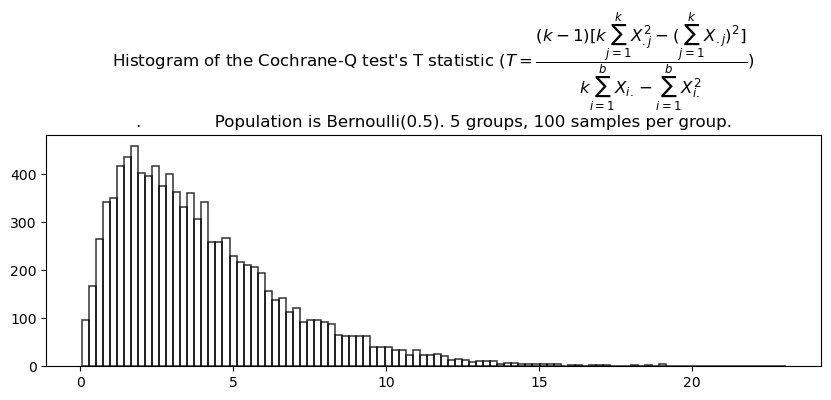
\includegraphics[width=0.52\textwidth]{fig15-Cochran Q mc1.png}
    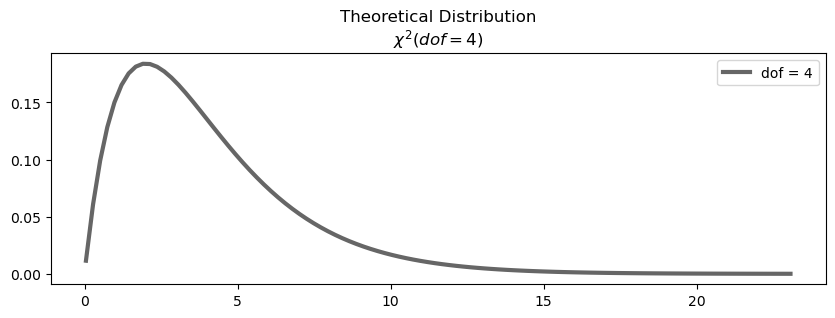
\includegraphics[width=0.45\textwidth]{fig15-Cochran Q mc2.png}
    \caption{The T statistic of Cochran's Q test and its theoretical chi-square distribution.}
    \label{fig:Cochran Q mc}
\end{figure}

\subsection{Hotelling's $T^2$ Test}
The Hotelling's $T^2$ test compares the mean of two multivariate populations.
Suppose we have two groups of samples from $N(\mu_{1},\sum)$ and $N(\mu_{2},\sum)$.
They share the same covariance matrix $\sum$. The null hypothesis is $H_{0}: \mu_{1}=\mu_{2}$
and the test statistic is:
\begin{equation}
    \label{deqn_ex14}
    T^2=n(\overline{x}-\mu)^{T}S^{-1}(\overline{x}-\mu)
\end{equation}

\noindent $S=\frac{1}{n-1}\sum_{i=1}^{n}(x_{i}-\overline{x})(x_{i}-\overline{x})^T$  is the grand covariance matrix.

If the dimensionality k=1, Hotelling's $T^2$ degenerates into the t distribution.
When $K \geq 2$, it is a multivariate generalization of the t distribution. The Hotelling\_T2\_Test
class verifies the $T^2$ sampling distribution (Figure \ref{fig:Hotelling T mc}).

\lstset{
    basicstyle=\footnotesize,
    xleftmargin=-1em,aboveskip=0.5em,belowskip=0.5em
}
\begin{lstlisting}[language=python]
    Hotelling_T2_Test(n=50,k=2,N=1000).run()
    # n : the sample size in each class.
    # k : data dimension.
    # N : how many MC experiments to run.
    \end{lstlisting}

\begin{figure}[htbp]
    \centering
    \vspace{-0.5em}
    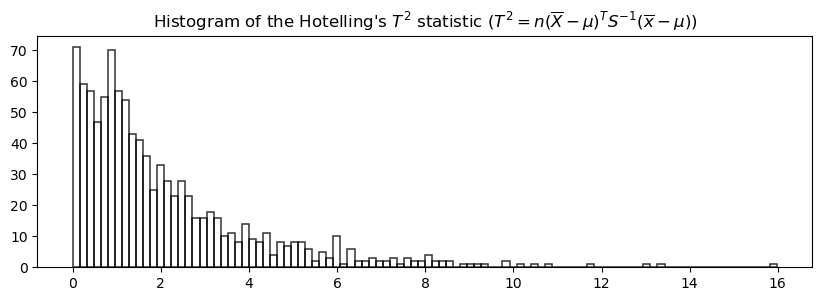
\includegraphics[width=0.45\textwidth]{fig16-Hotelling T mc1.png}
    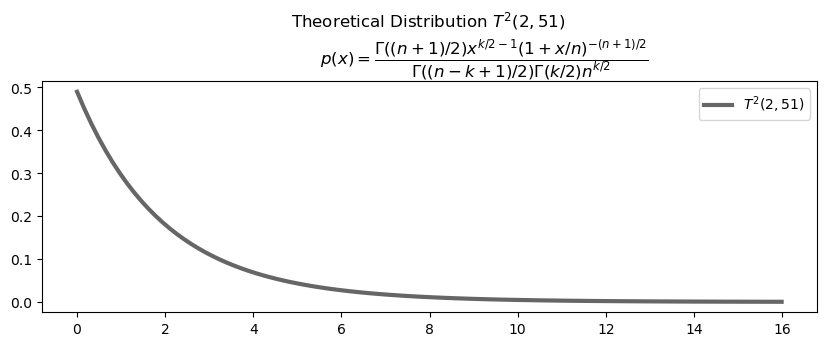
\includegraphics[width=0.45\textwidth]{fig16-Hotelling T mc2.png}
    \caption{The $T^2$ statistic of Hotelling's test.}
    \label{fig:Hotelling T mc}
\end{figure}

\subsection{Central Limit Theorem}
The Central Limit Theorem (CLT) is a fundamental theory in statistics. It explains why so many physical
phenomena follow the normal distribution. No matter the underlying distribution, the sum/average of enough
i.i.d. r.v.s. will approach the normal distribution. The Clt class provides these underlying distributions
to test CLT. (1) uniform, (2) exponential, see Figure \ref{fig17-clt mc1}, (3) Poisson, (4) coin, i.e., Bernoulli with
$p = 0.5$, (5) tampered coin, e.g., Bernoulli with p = 0.8, (6) dice, i.e., $p(k) = 1/6$, (7) tampered dice, e.g.,
$p(k=6) > 1/6$. See Figure \ref{fig17-clt mc2}.

\lstset{
    basicstyle=\scriptsize,
    xleftmargin=-1em,,aboveskip=0.5em,belowskip=0.5em
}
\begin{lstlisting}[language=python]
    Clt(underlying_dist='bernoulli',n=[1,2,5,20],N=10000).run()
    # underlying_dist : base/undeyling/atom distribution. 
    #     'uniform' - a uniform distribution U(-1,1) is used.
    #     'expon' - an exponential distribution Expon(1) is used.
    #     'poisson' - poisson distribution PI(1) is used.
    #     'coin' / 'bernoulli' - {0:0.5,1:0.5}.
    #     'tampered_coin' - {0:0.2,1:0.8}.
    #     'dice' - {1:1/6,2:1/6,3:1/6,4:1/6,5:1/6,6:1/6}
    #     'tampered_dice' - {1:0.1,2:0.1,3:0.1,4:0.1,5:0.1,6:0.5} 6 is more likely.
    #      None - use 0-1 distribution {0:0.5,1:0.5} by default.
    # n : sample size to be averaged over / summed up. Can be an array / list, user can check how the 
    #     histogram changes with sample size.
    # N : how many MC experiments to run.
    \end{lstlisting}

\begin{figure*}[!t]
    \centering
    \subfloat[]{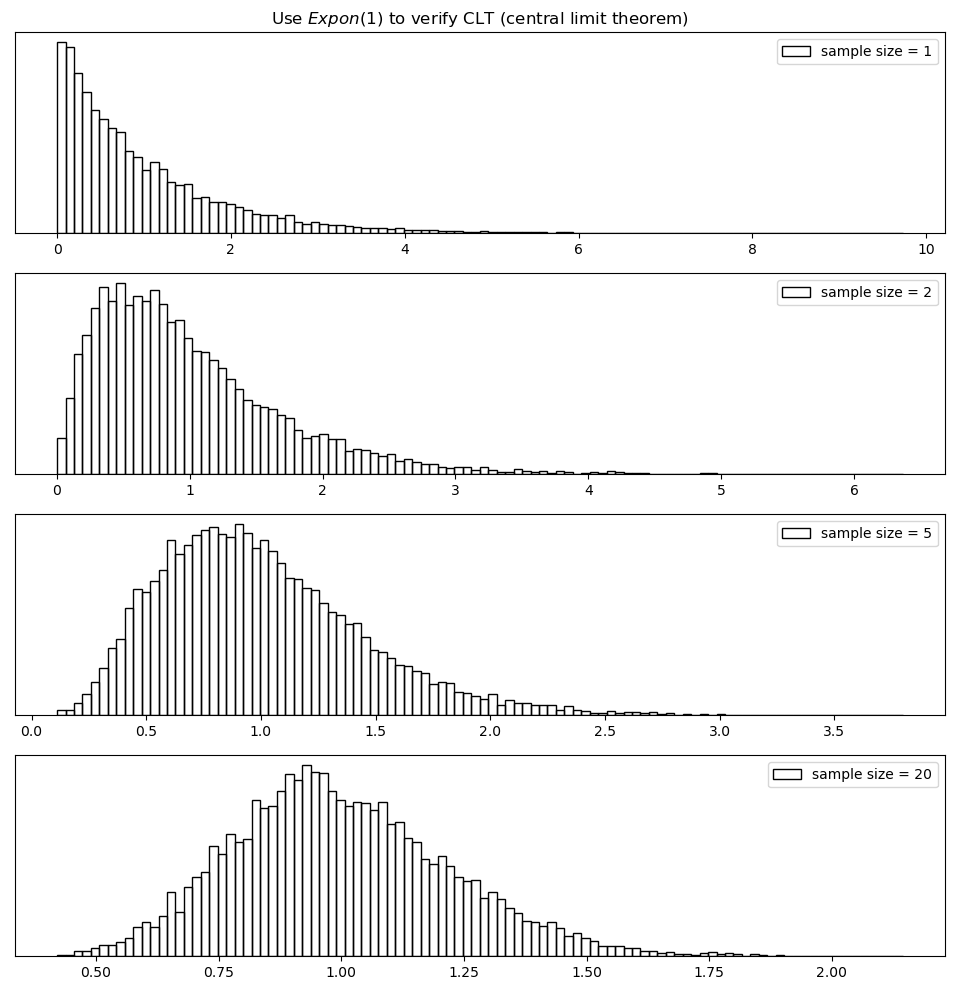
\includegraphics[width=0.47\textwidth]{fig17-clt mc1.png}%
        \label{fig17-clt mc1}}
    \hfil
    \subfloat[]{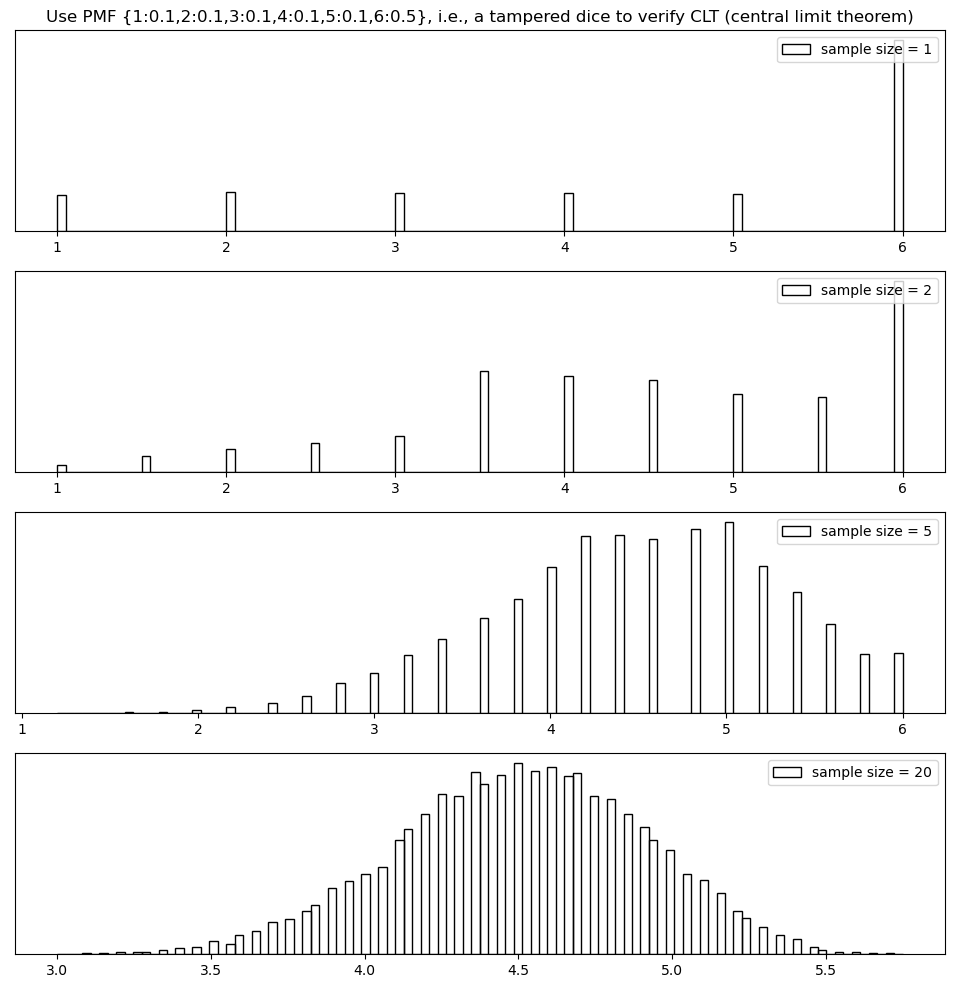
\includegraphics[width=0.47\textwidth]{fig17-clt mc2.png}%
        \label{fig17-clt mc2}}
    \caption{Use the exponential (a) and a tampered dice (e.g., six has a higher probability) (b) to verify CLT.}
    \label{fig:clt mc}
\end{figure*}

\bibliographystyle{elsarticle-num}
\bibliography{bibliography.bib}
\end{document}